Untuk membandingkan performa navigasi secara visual, Gambar~\ref{fig:visual_integrasi} menampilkan lintasan tiga mode operasi (\emph{fusion}, \emph{vision}, dan GPS) terhadap \emph{ground truth} DLIO pada rute pendek.

\begin{figure}[H]
    \centering
    \begin{subfigure}[b]{0.90\textwidth}
        \centering
        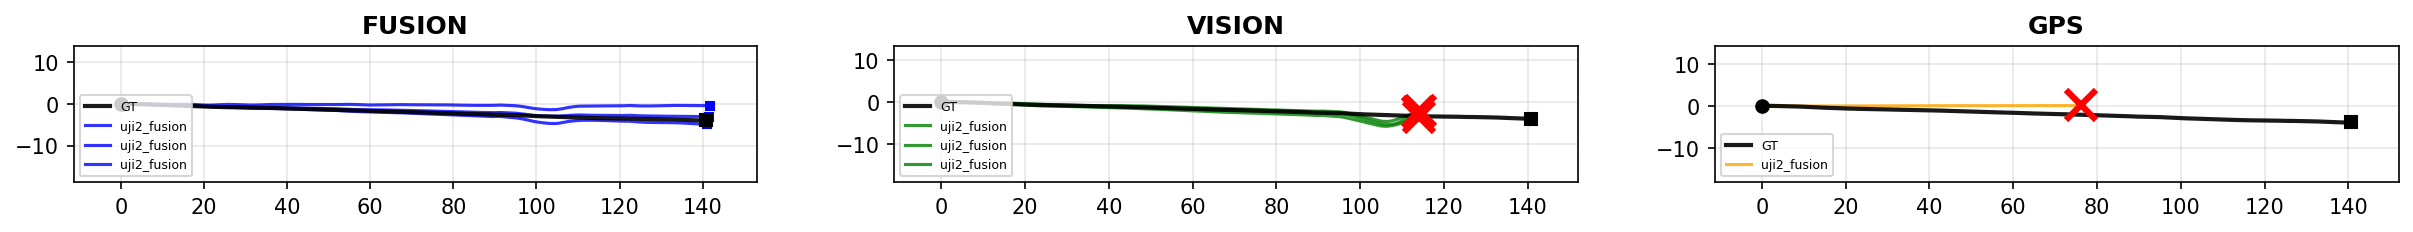
\includegraphics[width=\textwidth]{gambar/validation_trajectory_lurus.png}
        \caption{Skenario jalan lurus}
        \label{fig:visual_lurus}
    \end{subfigure}
    \hfill
    \begin{subfigure}[b]{0.90\textwidth}
        \centering
        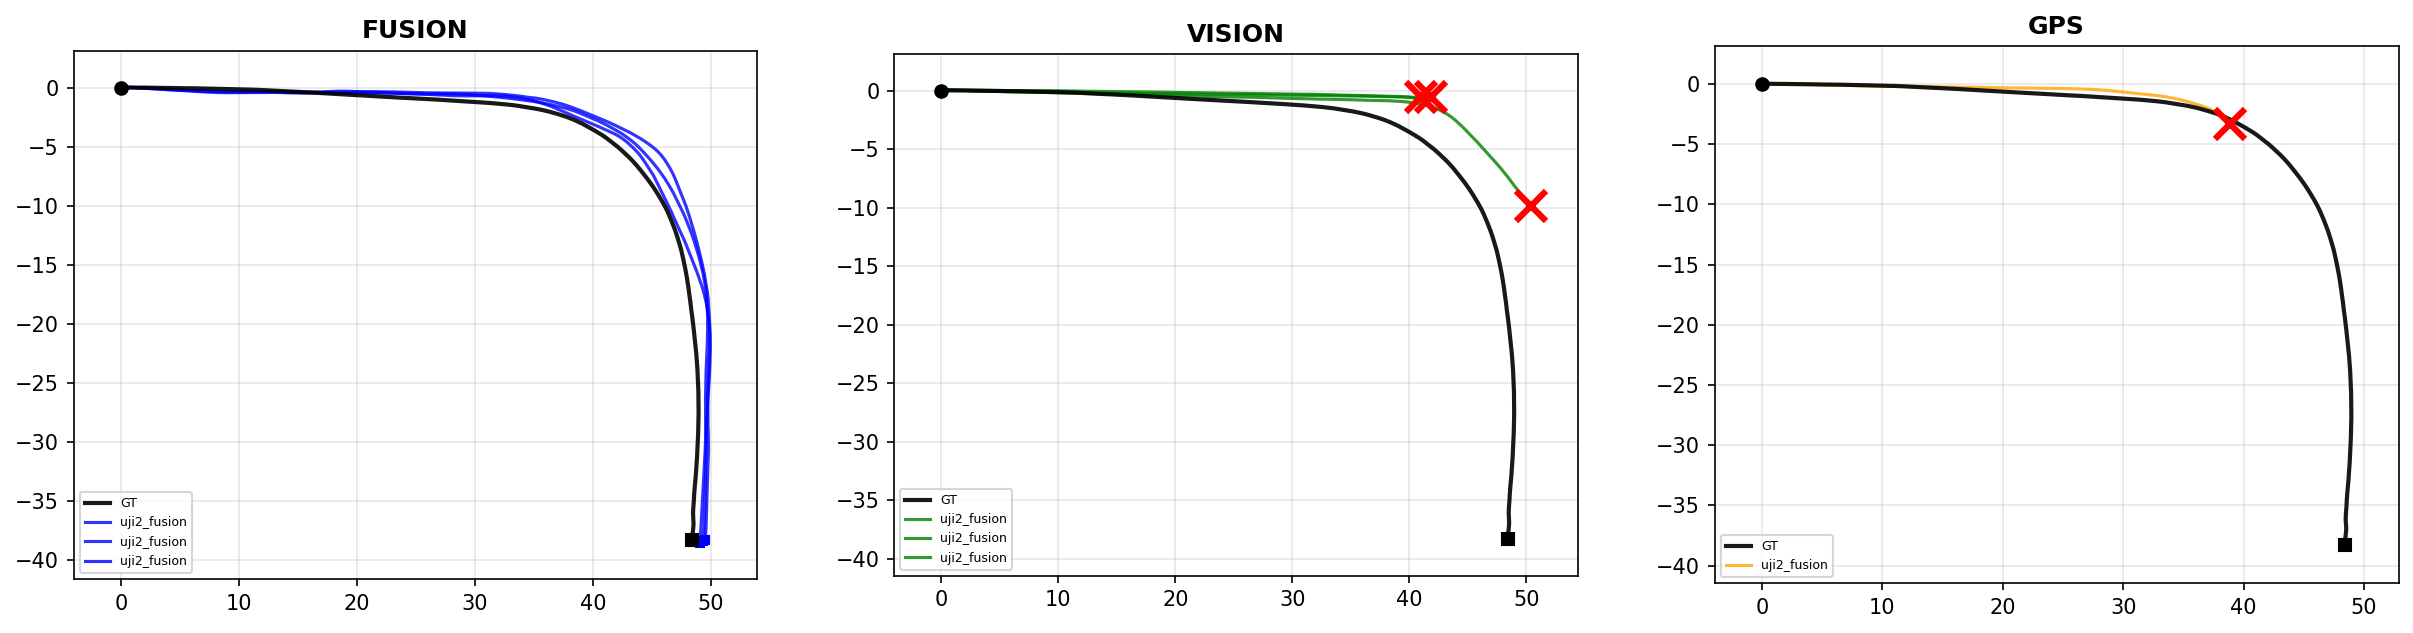
\includegraphics[width=\textwidth]{gambar/validation_trajectory_belok.png}
        \caption{Skenario jalan belok}
        \label{fig:visual_belok}
    \end{subfigure}
    \caption{Perbandingan navigasi pada tiga mode operasi (\emph{fusion}, \emph{vision}, dan GPS) terhadap \emph{ground truth} DLIO pada rute pendek.}
    \label{fig:visual_integrasi}
\end{figure}

\subsubsection{Pengujian Lintasan Jarak Jauh}
\label{sec:uji_jarak_jauh}

Untuk mengevaluasi kemampuan sistem dalam bernavigasi secara otonom pada jarak yang jauh, dilakukan pengujian dengan mode integrasi penuh (\emph{fusion}) pada lintasan sepanjang 3.674~m selama 31,99 menit. Tabel~\ref{tab:uji_jarak_jauh} merangkum hasil pengujian.

\begin{table}[H]
\centering
\caption{Hasil pengujian lintasan jarak jauh}
\label{tab:uji_jarak_jauh}
\begin{tabular}{l c}
\hline
\textbf{Parameter} & \textbf{Nilai} \\
\hline
Panjang lintasan DLIO (m)       & 3.674,03 \\
Panjang lintasan KF (m)         & 3.674,21 \\
Selisih panjang (m)             & 0,19 (0,005\%) \\
RMSE KF vs DLIO (m)             & 1,08 \\
Deviasi maksimum (m)            & 1,99 \\
Kecepatan rata-rata (m/s)       & 1,91 (6,9 km/jam) \\
Durasi (menit)                  & 31,99 \\
\hline
\end{tabular}
\end{table}

Selisih panjang lintasan antara KF dan DLIO hanya 0,19~m dari total 3.674~m—atau 0,005\%—menunjukkan bahwa sistem mampu melacak posisi secara konsisten tanpa akumulasi galat yang signifikan sepanjang perjalanan. RMSE posisi tercatat 1,08~m dengan deviasi maksimum 1,99~m.

Gambar~\ref{fig:uji2_full} dan~\ref{fig:uji2_zoom} menampilkan lintasan penuh dan cuplikan segmen.

\begin{figure}[H]
    \centering
    \begin{subfigure}[b]{0.48\textwidth}
        \centering
        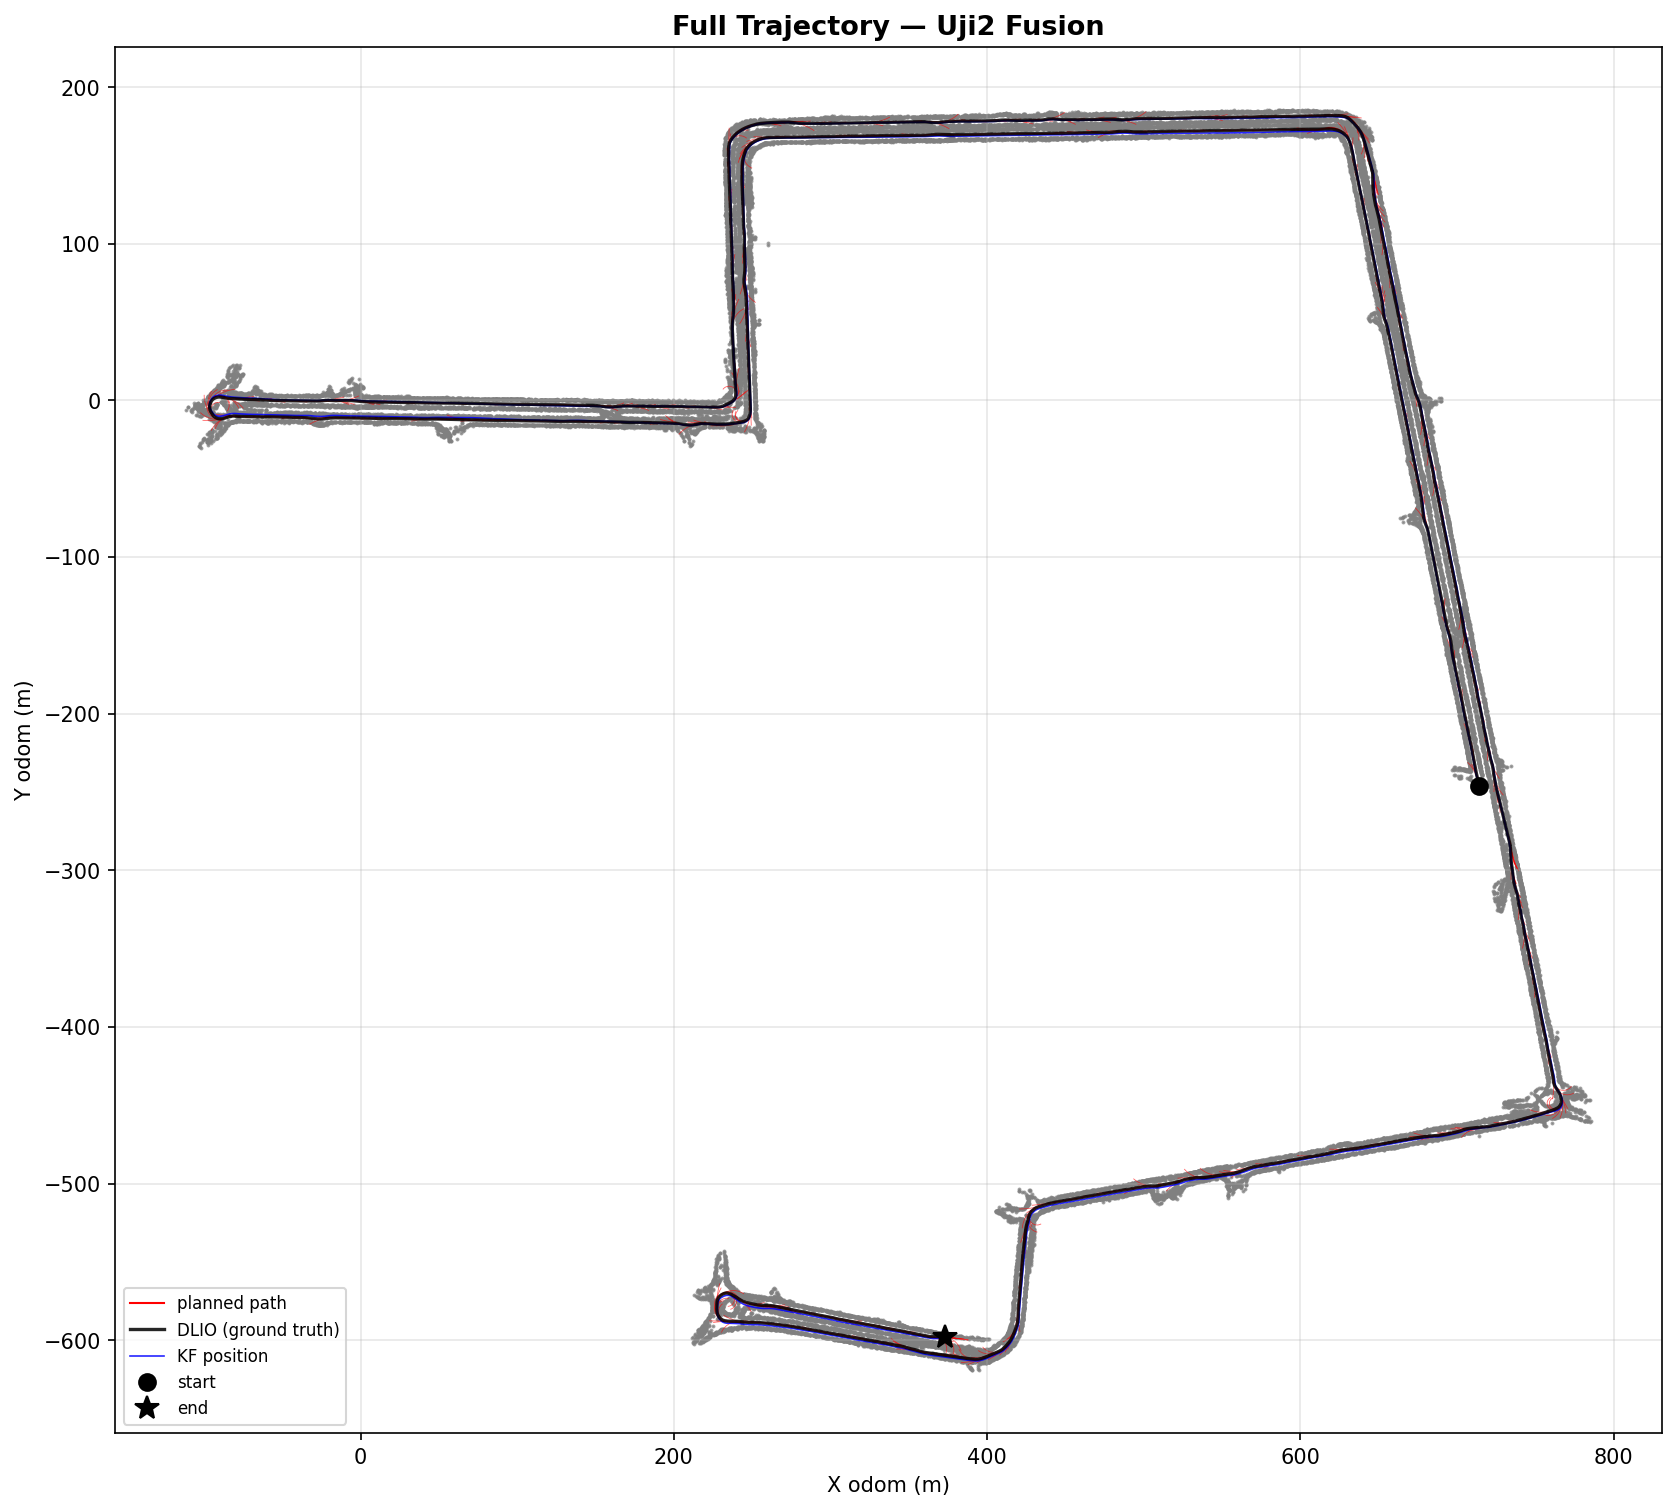
\includegraphics[width=\textwidth]{gambar/uji2_fusion_full.png}
        \caption{Lintasan penuh}
        \label{fig:uji2_full}
    \end{subfigure}
    \hfill
    \begin{subfigure}[b]{0.48\textwidth}
        \centering
        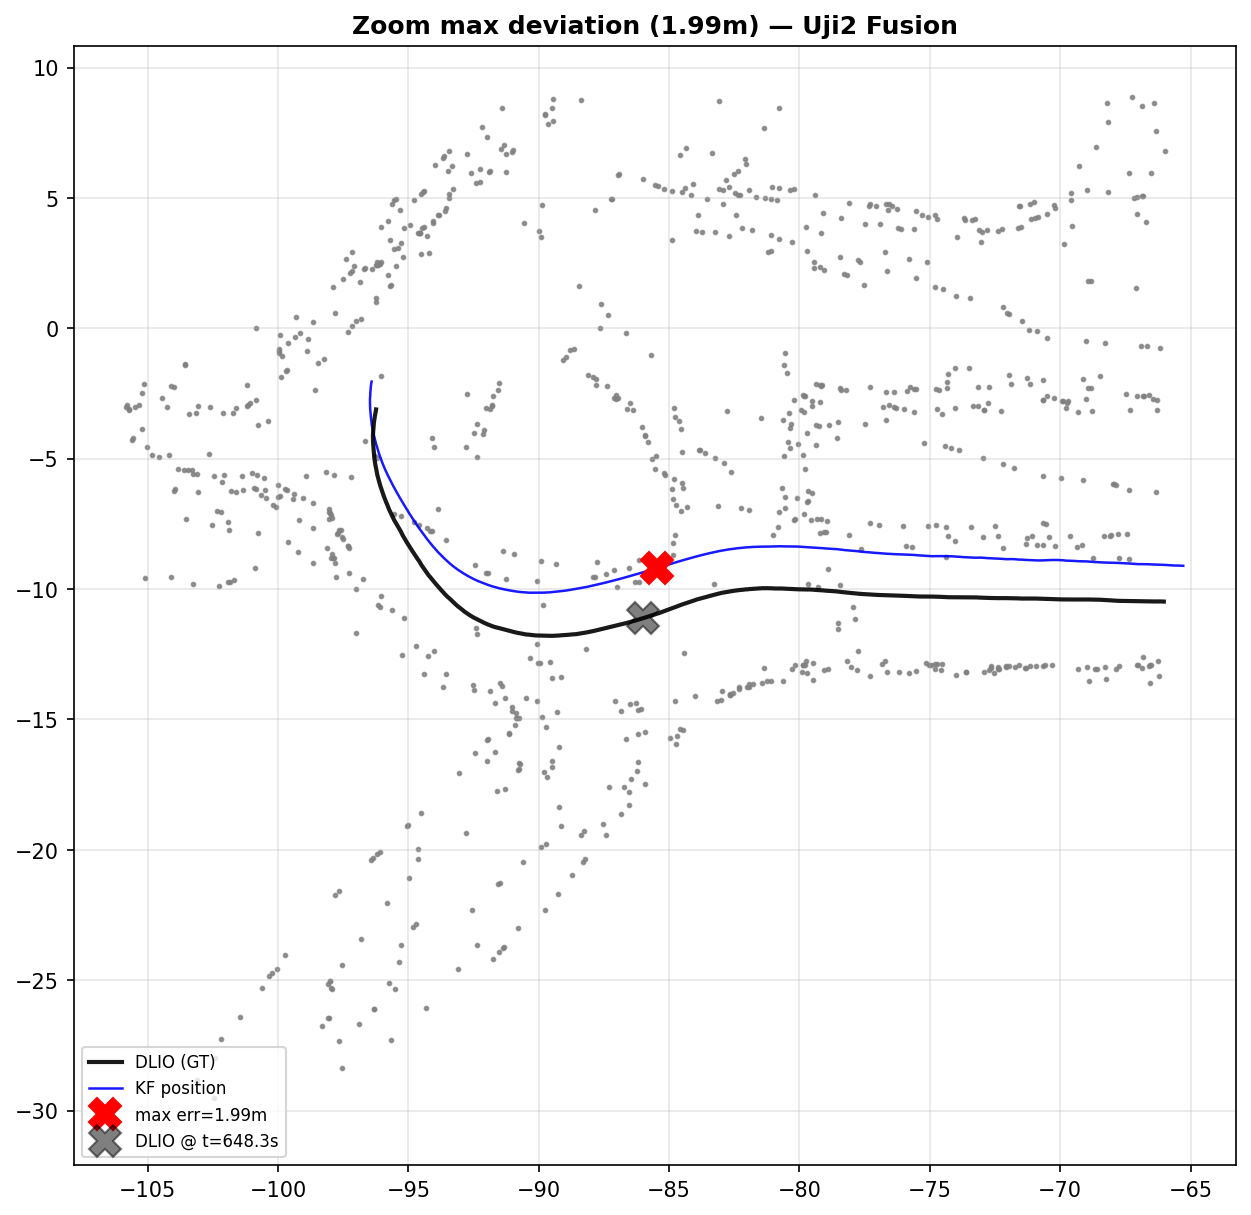
\includegraphics[width=\textwidth]{gambar/uji2_fusion_full_zoom.png}
        \caption{Cuplikan segmen}
        \label{fig:uji2_zoom}
    \end{subfigure}
    \caption{Lintasan KF terhadap DLIO pada pengujian \emph{autonomous} jarak jauh 3,7~km.}
    \label{fig:uji2_far}
\end{figure}

\subsubsection{Keberhasilan Penyelesaian Rute}
\label{sec:completion_rate}

Keberhasilan penyelesaian rute diukur untuk setiap metode operasi pada dua rute yang berbeda (lurus dan belok).
Rute lurus memiliki panjang 141.15 meter, sedangkan rute belok memiliki panjang 78.52 meter.
Setiap metode diuji sebanyak 3 kali pada masing-masing rute kecuali metode GPS yang hanya diuji 1 kali pada setiap rute karena keterbatasan data titik acuan KML/GeoJSON yang tersedia.

\begin{table}[H]
\centering
\caption{Keberhasilan penyelesaian rute setiap metode pada rute lurus dan belok}
\label{tab:completion_rate}
\begin{tabular}{l c c c}
\hline
\textbf{Metode} & \textbf{Rute Lurus} & \textbf{Rute Belok} & \textbf{Total} \\
\hline
\emph{Fusion}  & 3/3 & 3/3 & \textbf{6/6 (100\%)} \\
\emph{Vision}  & 0/3 & 0/3 & 0/6 (0\%) \\
GPS            & 0/1 & 0/1 & 0/2 (0\%) \\
\hline
\end{tabular}
\end{table}

Metode \emph{fusion} berhasil menyelesaikan semua percobaan pada kedua rute, menunjukkan bahwa integrasi segmentasi visual dengan \emph{waypoint} GPS menghasilkan navigasi yang andal.
Sebaliknya, metode \emph{vision} dan GPS gagal menyelesaikan seluruh percobaan.

\subsubsection{Akurasi Destinasi}
\label{sec:dest_accuracy}

Akurasi destinasi mengukur seberapa dekat kendaraan berhasil mencapai titik tujuan yang diinginkan, yang merupakan indikator penting untuk menilai efektivitas navigasi. 
Tabel~\ref{tab:dest_accuracy} menyajikan hasil pengukuran akurasi destinasi untuk setiap metode pada kedua rute.

\begin{table}[H]
\centering
\caption{Akurasi destinasi setiap metode pada rute lurus dan belok}
\label{tab:dest_accuracy}
\begin{tabular}{l c c}
\hline
\textbf{Metode} & \textbf{Error Destinasi Rute Lurus (m)} & \textbf{Error Destinasi Rute Belok (m)} \\
\hline
\emph{Fusion}  & 0,7 & 0,5 \\
\emph{Vision}  & -- & -- \\
GPS            & -- & -- \\
\hline
\end{tabular}
\end{table}

Metode \emph{fusion} mencapai akurasi destinasi di bawah 1 meter pada kedua rute, menunjukkan presisi tinggi dalam mencapai titik tujuan.
Sedangkan metode lainnya gagal menyelesaikan rute sehingga tidak dapat diukur akurasi destinasi.

\subsubsection{Ketahanan terhadap Gangguan GPS}
\label{sec:noise_robustness}

Ketahanan sistem terhadap gangguan GPS diuji dengan membandingkan performa pada dua kondisi navigasi yang berbeda dengan rute yang sama.
Pada kondisi pertama, sistem beroperasi tanpa injeksi kebisingan GPS ($\sigma = 0$), sedangkan pada kondisi kedua, sistem beroperasi dengan injeksi kebisingan Gaussian pada data GPS ($\sigma = 0,2$ m) untuk mensimulasikan kondisi degradasi sinyal GPS.
Pengujian diukur berdasarkan Root Mean Square Error (RMSE) antara lintasan yang dihasilkan dengan metode Kalman Filter terhadap metode pembanding DLIO.
Pada kondisi tanpa gangguan GPS, RMSE mencapai 0,404 meter, sedangkan pada kondisi dengan gangguan GPS, RMSE meningkat menjadi 0,705 meter.
Sehingga terlihat bahwa injeksi kebisingan GPS meningkatkan RMSE sebesar 74,6\%, namun sistem tetap mampu bernavigasi sepanjang rute dengan aman tanpa ada masalah.
